\documentclass[12pt]{article}

\usepackage{amsmath,amsthm,amsfonts,amssymb,amsxtra}
\usepackage{pgf,tikz}
\usetikzlibrary{arrows}
\renewcommand{\theenumi}{(\alph{enumi})} 
\renewcommand{\labelenumi}{\theenumi}

\pagestyle{empty}
\setlength{\textwidth}{7in}
\setlength{\oddsidemargin}{-0.5in}
\setlength{\topmargin}{-1.0in}
\setlength{\textheight}{9.5in}

\theoremstyle{definition}
\newtheorem{problem}{Problem}

\makeatletter
\newcommand*{\radiobutton}{%
  \@ifstar{\@radiobutton0}{\@radiobutton1}%
}
\newcommand*{\@radiobutton}[1]{%
  \begin{tikzpicture}
    \pgfmathsetlengthmacro\radius{height("X")/2}
    \draw[radius=\radius] circle;
    \ifcase#1 \fill[radius=.6*\radius] circle;\fi
  \end{tikzpicture}%
}
\makeatother

\begin{document}

\noindent{\large\bf MATH 122}\hfill{\large\bf Exam \#3.}\hfill{\large\bf Fall 2018}\hfill{\large\bf Page 1/5}\hrule

\bigskip
\begin{center}
  \begin{tabular}{|ll|}
    \hline & \cr
    {\bf Name: } & \makebox[12cm]{\hrulefill}\cr & \cr
    {\bf VIP ID:} & \makebox[12cm]{\hrulefill}\cr & \cr
    \hline
  \end{tabular}
\end{center}
\begin{itemize}
\item Write your name and your VIP ID in the space provided above.
\item The test has five (5) pages, including this one.
\item You must show sufficient work to justify all answers unless otherwise stated in the problem.  Correct answers with inconsistent
  work may not be given credit.
\item Credit for each problem is given in parentheses at the right of the problem number.
\item No books, or notes may be used on this test.
\item An approved calculator may be used on this test.
\end{itemize}
\hrule

\begin{center}
  \begin{tabular}{|c|c|c|}
    \hline
    &&\cr
    {\large\bf Page} & {\large\bf Max.~points} & {\large\bf Your points} \cr
    &&\cr
    \hline
    &&\cr
    {\Large 2} & \Large 20 & \cr
    &&\cr
    \hline
    &&\cr
    {\Large 3} & \Large 20 & \cr
    &&\cr
    \hline
    &&\cr
    {\Large 4} & \Large 40 & \cr
    &&\cr
    \hline
    &&\cr
    {\Large 5} & \Large 20 & \cr
    &&\cr
    \hline\hline
    &&\cr
    {\large\bf Total} & \Large 100 & \cr
    &&\cr
    \hline
  \end{tabular}
\end{center}
\newpage

%%%%%%%%%%%%%%%%%%%%%%%%%%%%%%%%%%%%% Page 2
\noindent{\large\bf MATH 122}\hfill{\large\bf Exam \#3.}\hfill{\large\bf Fall 2018}\hfill{\large\bf Page 2/5}\hrule

\bigskip
\begin{problem}[10 pts]
The function $f(x) = x^4 - 5x^3 + 11x$ has a critical point at $x=1$.  Identify what kind of critical point it is.
\begin{itemize}
\item[\radiobutton] $f(x)$ has a local maximum at $x=1$.
\item[\radiobutton] $f(x)$ has a local minimum at $x=1$.
\item[\radiobutton] $x=1$ is neither maximum nor minimum of $f(x)$.
\end{itemize}
\end{problem}
\vspace{5cm}
\hrule
\begin{problem}[10 pts]
  Find intervals of increase/decrease and concavity of the function
  \begin{equation*}
    f(x) = 2x^3 + 3x^2-180x+9.
  \end{equation*}
\end{problem}
\newpage

%%%%%%%%%%%%%%%%%%%%%%%%%%%%%%%%%%%%% Page 3
\noindent{\large\bf MATH 122}\hfill{\large\bf Exam \#3.}\hfill{\large\bf Fall 2018}\hfill{\large\bf Page 3/5}\hrule

\bigskip
\begin{problem}[10 pts]
Concerning the graph of the function below, which of the following statements is true?
\begin{center}
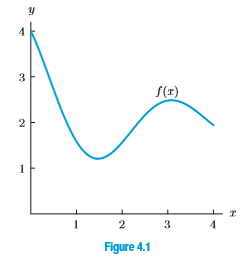
\includegraphics{3graph3}
\end{center}
\begin{itemize}
\item[\radiobutton] The derivative is zero at two values of $x$, both being local maxima.
\item[\radiobutton] The derivative is zero at two values of $x$, one is a local maximum, while the other is a local minimum.
\item[\radiobutton] The derivative is zero at two values of $x$, one is a local maximum on the interval, while the other is neither a local maximum nor a minimum.
\item[\radiobutton] The derivative is zero at two values of $x$, one is a local minimum on the interval, while the other is neither a local maximum nor a minimum.
\item[\radiobutton] The derivative is zero only at one value of $x$, where it is a local minimum.
\end{itemize}
\end{problem}

\hrule
\begin{problem}[10 pts]
Find the absolute maximum and the absolute minimum values of the function $f(x) = 2x^3 - 9x^2$ over the interval $-1 \leq x \leq 6$.
\end{problem}
\newpage

%%%%%%%%%%%%%%%%%%%%%%%%%%%%%%%%%%%%% Page 4
\noindent{\large\bf MATH 122}\hfill{\large\bf Exam \#3.}\hfill{\large\bf Fall 2018}\hfill{\large\bf Page 4/5}\hrule

\bigskip
\begin{problem}[10 pts]
  Suppose $P(t)$ is the number of individuals infected by a disease $t$ days after it was first detected. Interpret $P'(50)=200.$
\end{problem}
\vspace{2cm}
\hrule

\begin{problem}[10 pts]
  A baseball team plays in a stadium that holds 50,000 spectators.  With the ticket price at \$8 the average attendance
  has been 19,000.  When the price dropped to \$4, the average attendance rose to 25,000.  Find a linear demand function
  $D(q)$, where $q$ is the number of spectators.
\end{problem}
\vspace{4cm}
\hrule

\begin{problem}[10 pts]
  The total cost of producing $q$ units of good is given by $C(q) = 7.3q + 56000.$
  \begin{enumerate}
  \item What is the total cost of producing 4200 units?
    \vspace{2cm}
  \item What is the cost of the 4201st item?
  \end{enumerate}
  \vspace{2cm}
\end{problem}

\hrule
\begin{problem}[10 pts]
  The cost function of a product (in dollars) is given by $C(q) = 23.56 + 0.04q,$ where $q$ is the number of units
  sold.  What is the average cost of selling 200 units?
\end{problem}

\newpage

%%%%%%%%%%%%%%%%%%%%%%%%%%%%%%%%%%%%% Page 5
\noindent{\large\bf MATH 122}\hfill{\large\bf Exam \#3.}\hfill{\large\bf Fall 2018}\hfill{\large\bf Page 5/5}\hrule

\bigskip


\begin{problem}[10 pts]
  A manufacturer has been selling 1300 flat screen TVs a week at \$3600 each.  A market survey indicates that for each
  \$100 rebate offered to a buyer, the number of TVs sold increase by 100 per week.  The weekly cost function is given
  by $C(q) = 780000 + 1200q$.  What should be the rebate offered in order to maximize profit?
\end{problem}
\vspace{14cm}
\hrule

\begin{problem}[10 pts]
At a price of \$30 per ticket, a musical theater group can fill every seat in the theater, which has a capacity of 2800.  For every \$2.5 decrease in price, the number of people buying tickets increases by 175.  What ticket price maximizes revenue?
\end{problem}


\end{document}

%%% Local Variables:
%%% mode: latex
%%% TeX-master: t
%%% End:
